
\section{Requirements and Design Constraints}

\subsection{System Requirements}

To add custom content to the platform, a user must have a web browser and internet access. The user must also have access to modeling software or a means to provide 3D models to the website.

To view AR content, the user must have an augmented reality (AR) device. Each device may have different system requirements. AR devices such as the HoloLens or mobile devices operate as standalone hardware. Other AR devices may require a host computer to broadcast renderings to the device. Manufacturer details outline minimum specifications for a host computer, should it be needed.

For example, the Meta 2 headset requires a separate computer for model rendering and device hosting. As of November 2017, the Meta 2 has one of the highest recommended specifications among popular AR headsets. As a result, the recommended setup runs contemporary AR applications smoothly and with significant support. The minimum and recommended specifications are listed in Table \ref{table:metatwosystemrequirements}.

\begin{table}[H]
	\centering
	\begin{tabular}{ | c | c | c | }
		\hline
		& Minimum & Recommended \\ \hline
		OS & Windows 10 (64 bit) & 	Windows 10 (64 bit) \\ \hline
		CPU & Intel i7-4770 & Intel i7-6700 \\ \hline
		RAM & 8GB DDR3 & 16GB DDR4 \\ \hline
		GPU & NVIDIA GTX 960 & NVIDIA GTX 970 \\ \hline
		Hard Drive & 2GB Free Space & 2GB+ Free Space \\ \hline
		I/O Ports & 1X HDMI 1.4b and 2X USB 3.0 ports & 1X HDMI 1.4b and 2X USB 3.0 ports \\ \hline
		3D Engine & Unity 5.6 or higher & Unity 5.6 or higher \\ \hline
	\end{tabular}

	\caption{Meta 2 System Requirements}
	\label{table:metatwosystemrequirements}
\end{table}

More up to date requirements can be found on the Meta 2 website at: 
\url{https://buy.metavision.com/}

\subsection{Network Requirements}

Being able to take advantage of the features in this product needs a network
that is able to easily upload and download 3D models. The user needs to have
both their computer and AR viewer configured for network access.

\subsection{Development Environment Requirements}
% What are they? Is the system supposed to be cross-platform?
\begin{itemize}
	\item Windows 10 - To be able to develop for the HoloLens.
	\item Visual Studio 2017 Enterprise with ASP.NET MVS, Azure and Unity tools.
	\item Unity Personal
	\item HoloToolkit - Unity Set of tools for HoloLens development with Unity.
	\item Assimp library - For file conversion
	\item FBX SDK - For file conversion
	\item Android Studio
\end{itemize}


\subsection{Project Management Methodology}

The Senior Design I team structure for this project was self-organized. The team decided on the Agile development methodology, picked Brady Shimp as Scrum Master, and Cheldon Coughlen as Team Lead. The team had weekly status report meetings with client representatives and faculty advisors, Dr. McGough and Dr. Karlsson. At these meetings the team provided progress reports and discussed any design modifications or complications moving forward.\\

The Senior Design II team structure was refined from experiences, both good and bad, taken from the Senior Design I structure.  The team agreed that the Agile development methodology was too rigid and ineffective for a team with as many members and as many different times of availability. The team instead opted for a Feature Driven Development (FDD) methodology, that employed certain aspects of the Agile system that were deemed effective such as listing expected completion times for feature tasks and tracking productivity via the project board. This switch allowed the team to diversify into two sub-teams, one for mobile application development and one for continued web development, that each maintained structure and accountability within themselves. The decided leaders of the mobile application team and the continued web development team were Kenneth Petry and Brady Shimp, respectively.\\

Consistencies across both courses of Senior Design I and II were the Scrum style issue tracking, GitHub for the bulk project management tools, Google Team Drive for collaborative shared materials and presentation preparation, team communication through the Discord chat application, weekly status meetings with the project clients, and a structured task delegation system with a single point of authority.


\section{Product Backlog}

This project is intended to be a two-year development process. No features intended to be delivered after the first year were left incomplete or in the backlog. See Ch. \ref{ch:TODO} for a list of considered future developments. 

\subsection{Backlog Tracker}

During development, the backlog was managed using a GitHub project board. The GitHub platform was chosen because it also featured repository hosting and source control. 

The project board has four sections: "Backlog", "Work in Progress", "QA", and "Ready", as seen in Fig. 
~\ref{fig:ProjectTaskBoard}. Each sprint began by evaluating tasks and adding new tasks to the project board's "Backlog". Tasks would then be assigned to team members and moved to "Work in Progress". As tasks were completed, team members would select unassigned tasks to work on. Should tasks be prioritized or take longer than expected, other tasks may have been moved back to this backlog and made available for other developers. Completed tasks would be moved to "QA" for a quality assurance inspection by another teammate. Tasks that passed quality assurance would be moved to "Ready" by the evaluation. Tasks that did not pass quality assurance would be sent back to "Work in Progress" by the evaluation with constructive justification for the decision. 

\begin{figure}[H]
    \centering
    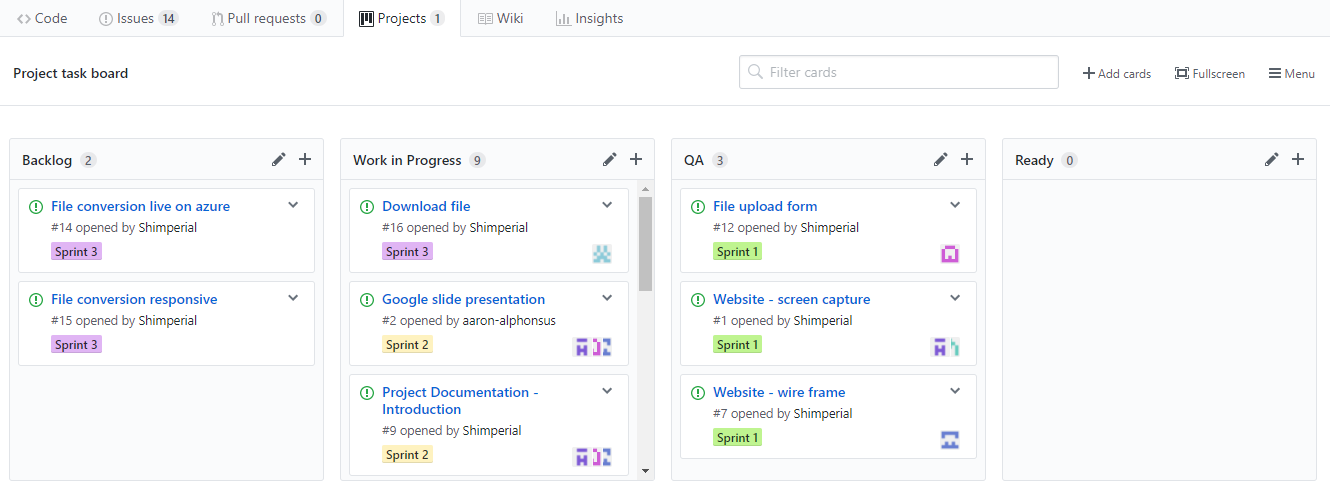
\includegraphics[width=\textwidth]{ProjectTaskBoard.png}
    \caption{Project Task Board}
    \label{fig:ProjectTaskBoard}
\end{figure}

Only the development team was granted permission to access the sprint log and backlog on GitHub. Documentation, presentations, and other communication provided insight regarding the status of the project to other interested parties. 


\section{Proof of Concept Results}

The development period occurring over Senior Design I focused on providing stakeholders a proof of concept so that they may conceptualize applications of the platform and drive requirements of the project in the future. To further lay this foundation, the development team hosted meetings with faculty to demonstrate AR and VR technology and its potential application in education. 

These efforts were successful in further refining requirements that would make the Augmented Education platform practical and applicable in classes taught by members of the client panel. The mobile application component of the project was added in December 2017 as a result. All relevant documentation was updated to reflect this major change. 

\section{Supporting Material}

All supporting materials have been included in Appendix \ref{ch:support}. Included is the Mobile Computing Grant which outlines SD Mine's long-term goals of this project. These goals have been used to define the direction and requirements of this project.
